
\section{BranchyNet Training}

%\begin{figure}
%	\centering
%	\captionsetup[subfigure]{justification=centering}
%	\subfloat[Train loss\label{fig:B-resnet-miniimagenet10-train-loss}]{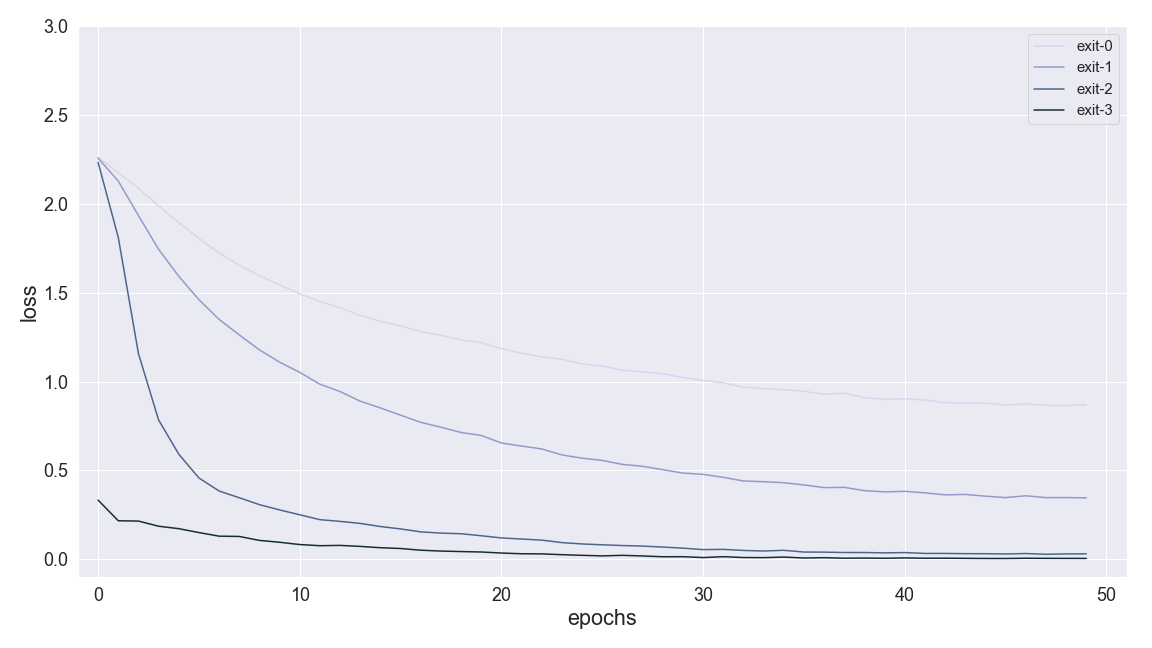
\includegraphics[width=.49\textwidth]{figures/bresnet_mini10/BResNet_train_loss_miniimagenet10.png}}
%	\subfloat[Test loss \label{fig:B-resnet-miniimagenet10-test-loss}]{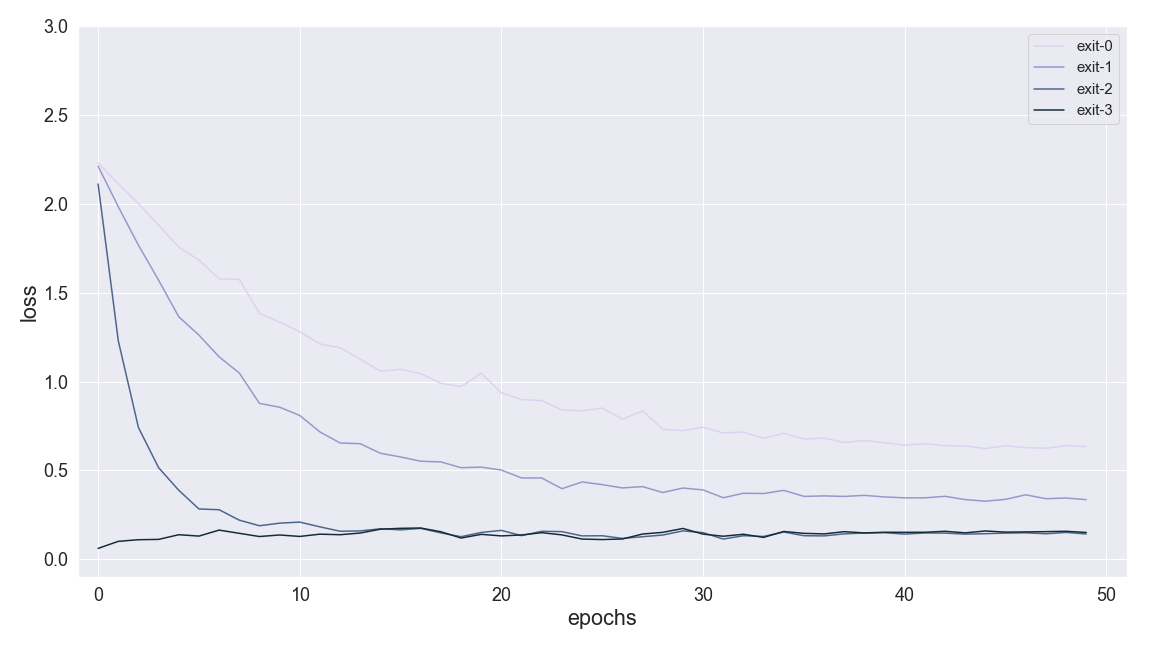
\includegraphics[width=.49\textwidth]{figures/bresnet_mini10/BResNet_test_loss_miniimagenet10.png}}
%	\hfill
%	\subfloat[Train accuracy\label{fig:B-resnet-miniimagenet10-train-acc}]{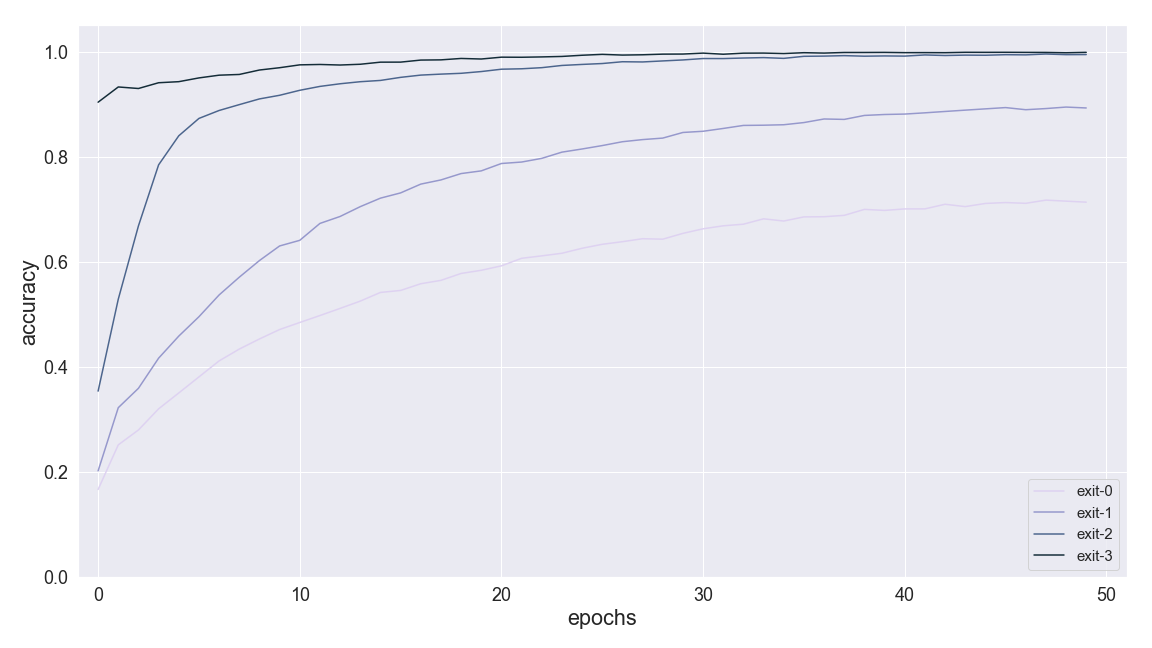
\includegraphics[width=.49\textwidth]{figures/bresnet_mini10/BResNet_train_acc_miniimagenet10.png}}
%	\subfloat[Test accuracy\label{fig:B-resnet-miniimagenet10-test-acc}]{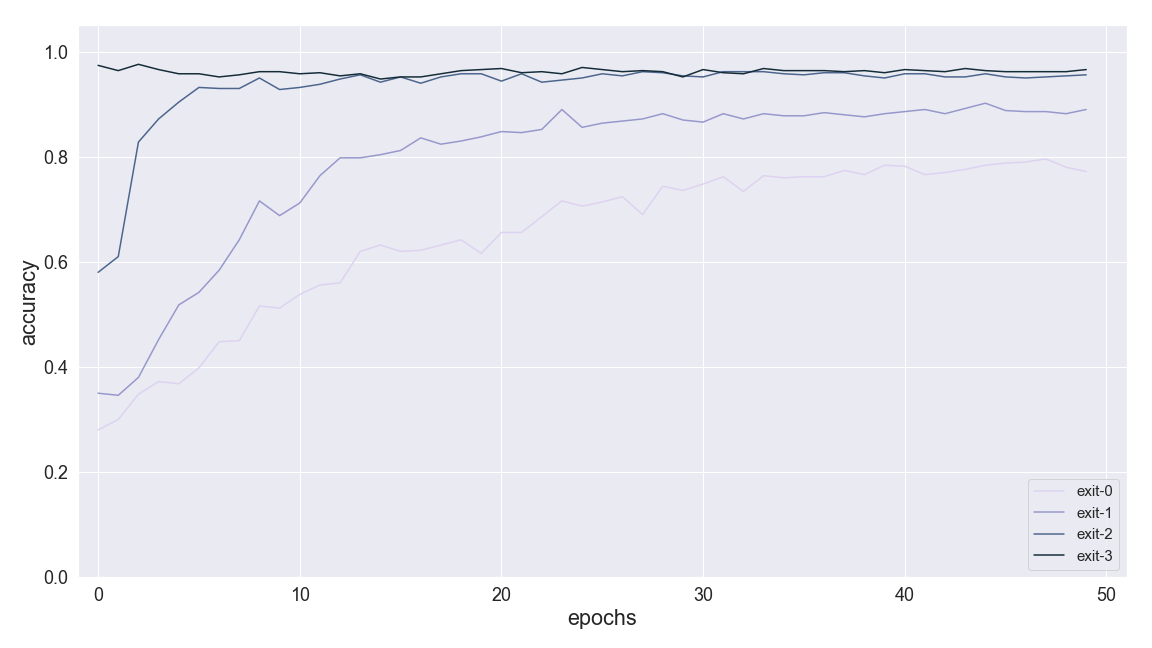
\includegraphics[width=.49\textwidth]{figures/bresnet_mini10/BResNet_test_acc_miniimagenet10.png}}
%	\caption[B-ResNet MiniImageNet10 Training summary]{Training summary shows the progression of model attributes over times of epochs, \protect\subref{fig:B-resnet-miniimagenet10-train-loss} train loss, \protect\subref{fig:B-resnet-miniimagenet10-test-loss} test loss, \protect\subref{fig:B-resnet-miniimagenet10-train-acc} train accuracy, \protect\subref{fig:B-resnet-miniimagenet10-test-acc}, test accuracy.}
%	\label{fig:B-resnet-miniimagenet-10}
%\end{figure}

Training B-\gls{resnet} and B-\gls{densenet} shows the importance of the densely connected layers for an early exiting model. The early exits of B-\gls{densenet} have a higher accuracy compared to B-\gls{resnet}, however B-\gls{resnet} last two exits are more accurate, see figure \ref{fig:b-net-miniimagenet-100}. 

\begin{figure}
	\centering
	\captionsetup[subfigure]{justification=centering}
	\subfloat[B-Resnet\label{fig:B-resnet-miniimagenet100}]{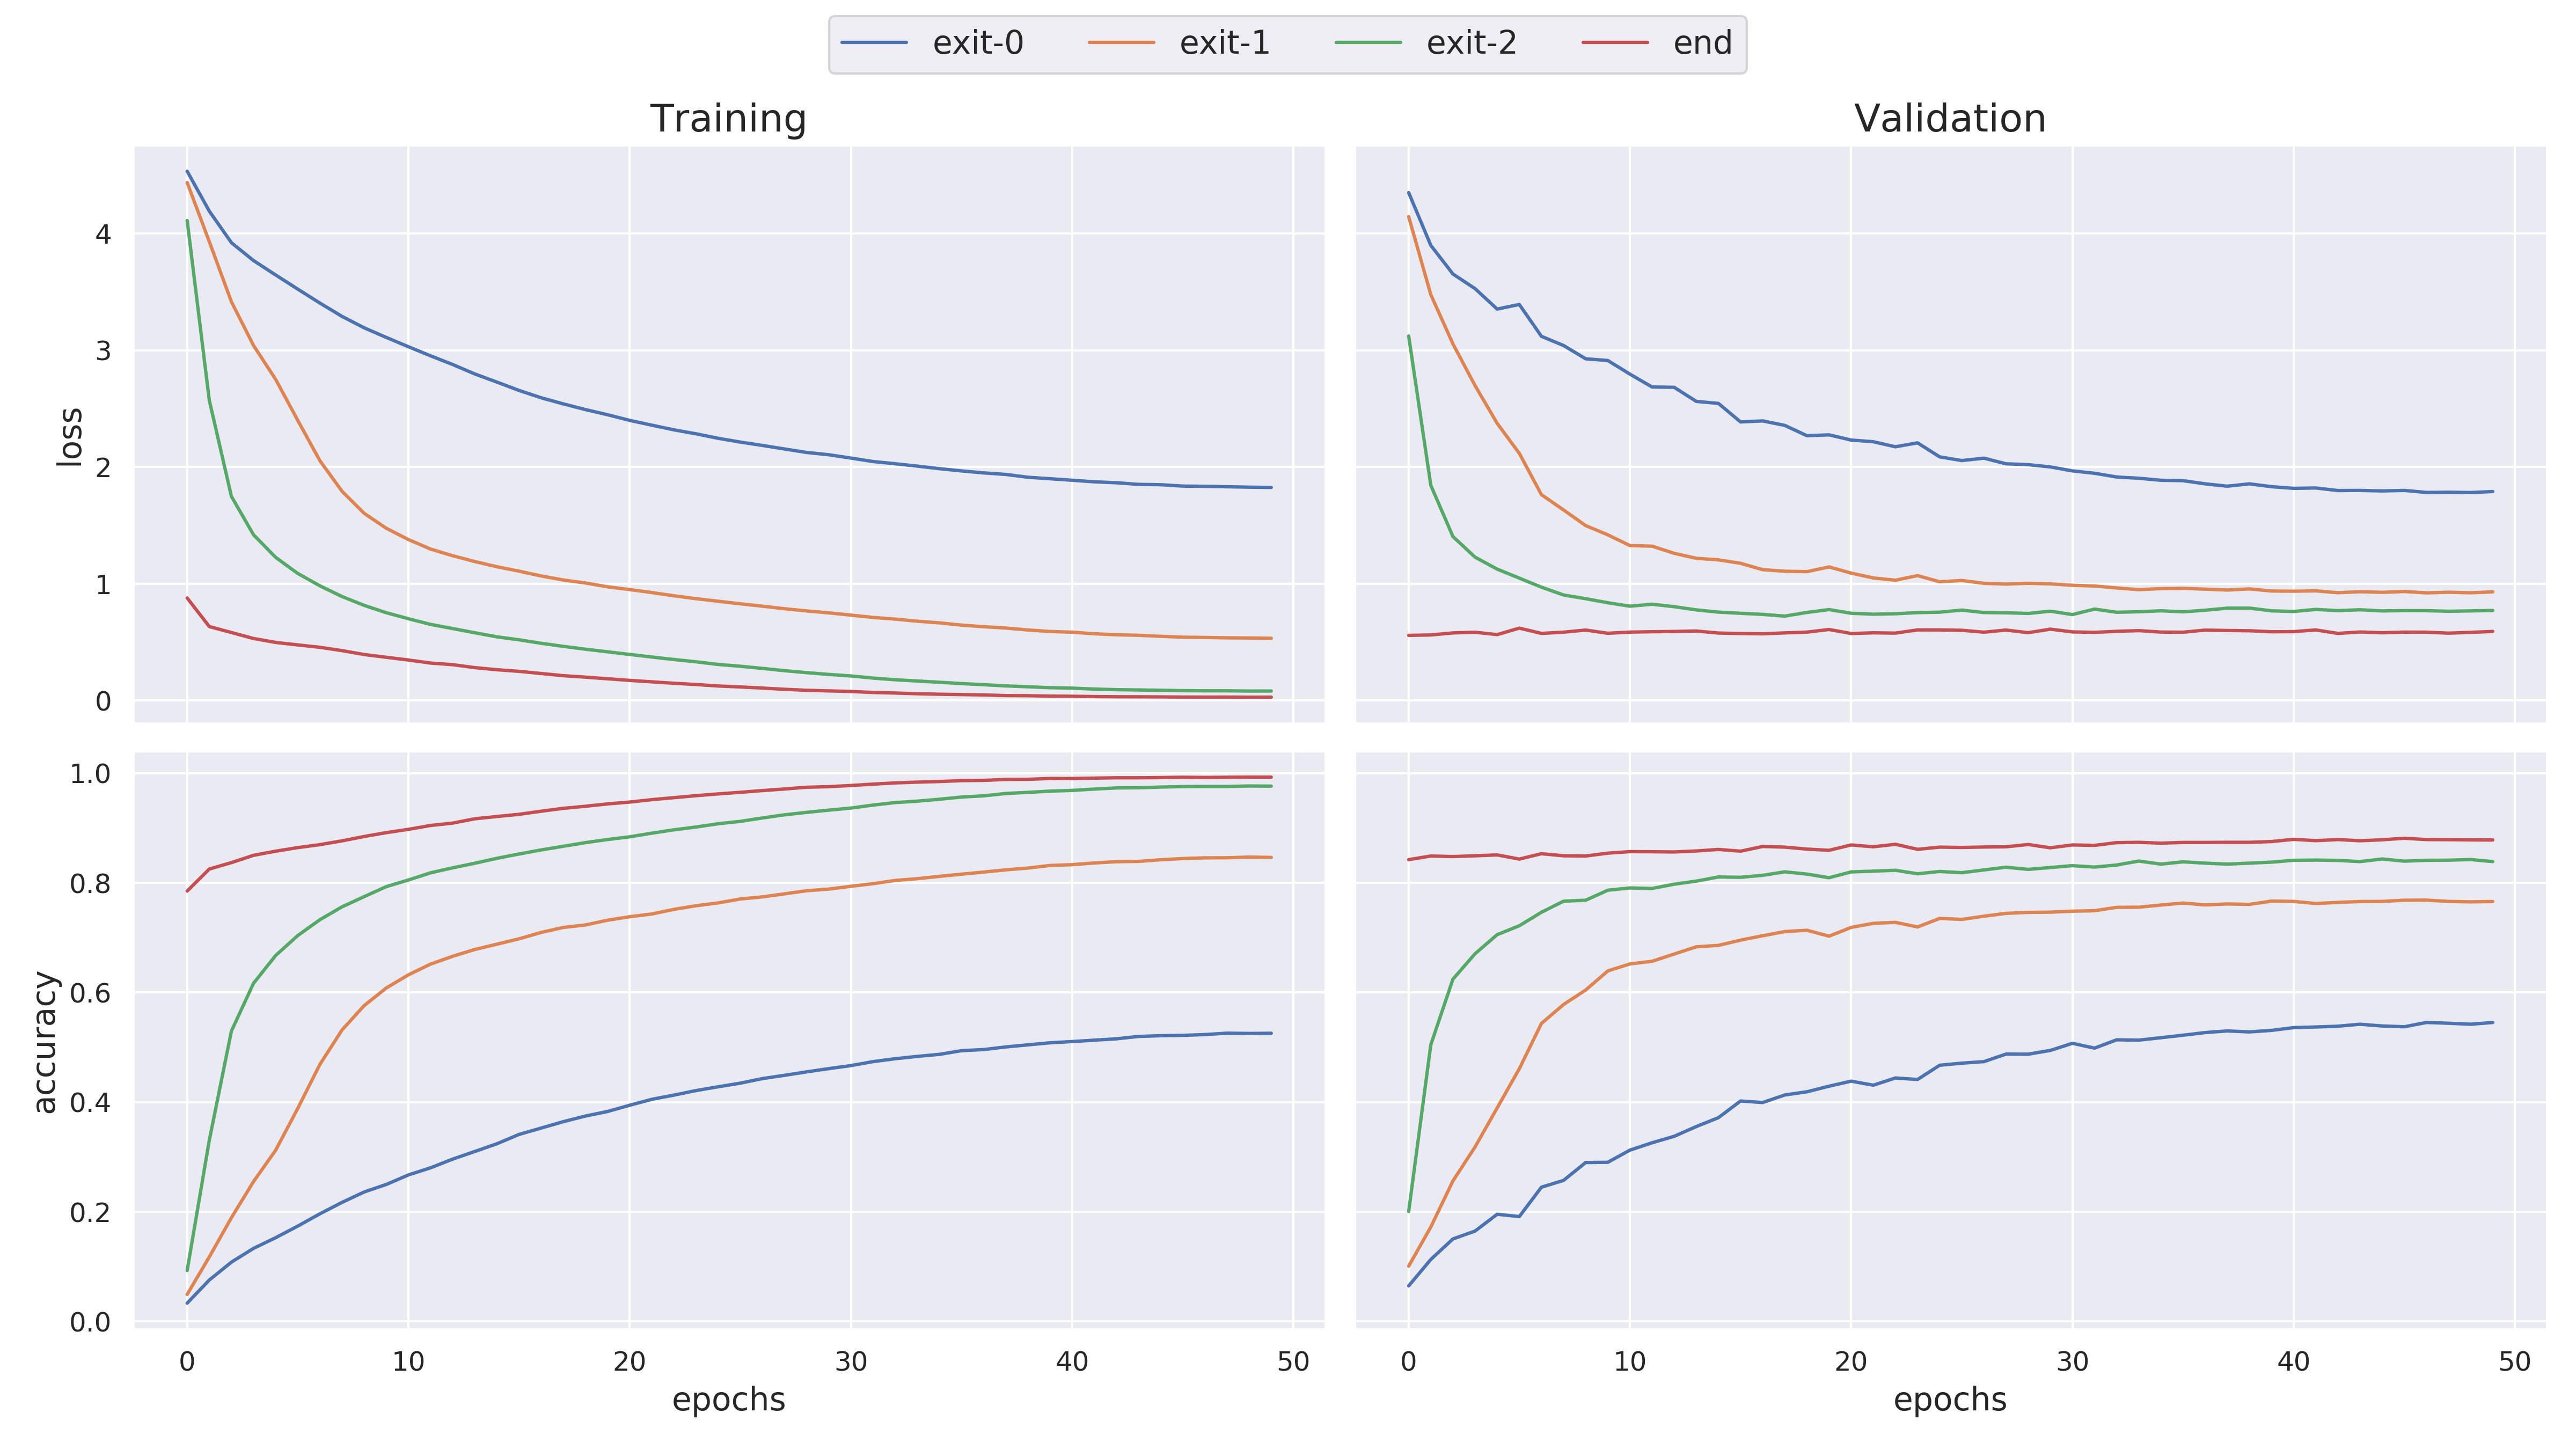
\includegraphics[width=\linewidth]{figures/training_plots/resnet_miniimagenet100}}
\end{figure}

The two last exits of \gls{resnet} are almost equally accurate. The resolution block of exit-2 are very deep, and the features becomes optimized for this classifier, hence not much gain in accuracy is obtained by running the early exit model all the way to the end. \gls{densenet} on the other hand always have an accuracy gain by continuing the inference process.    

\begin{figure}
	%\ContinuedFloat
	\captionsetup[subfigure]{justification=centering}
	\subfloat[B-DenseNet\label{fig:B-densenet-miniimagenet100}]{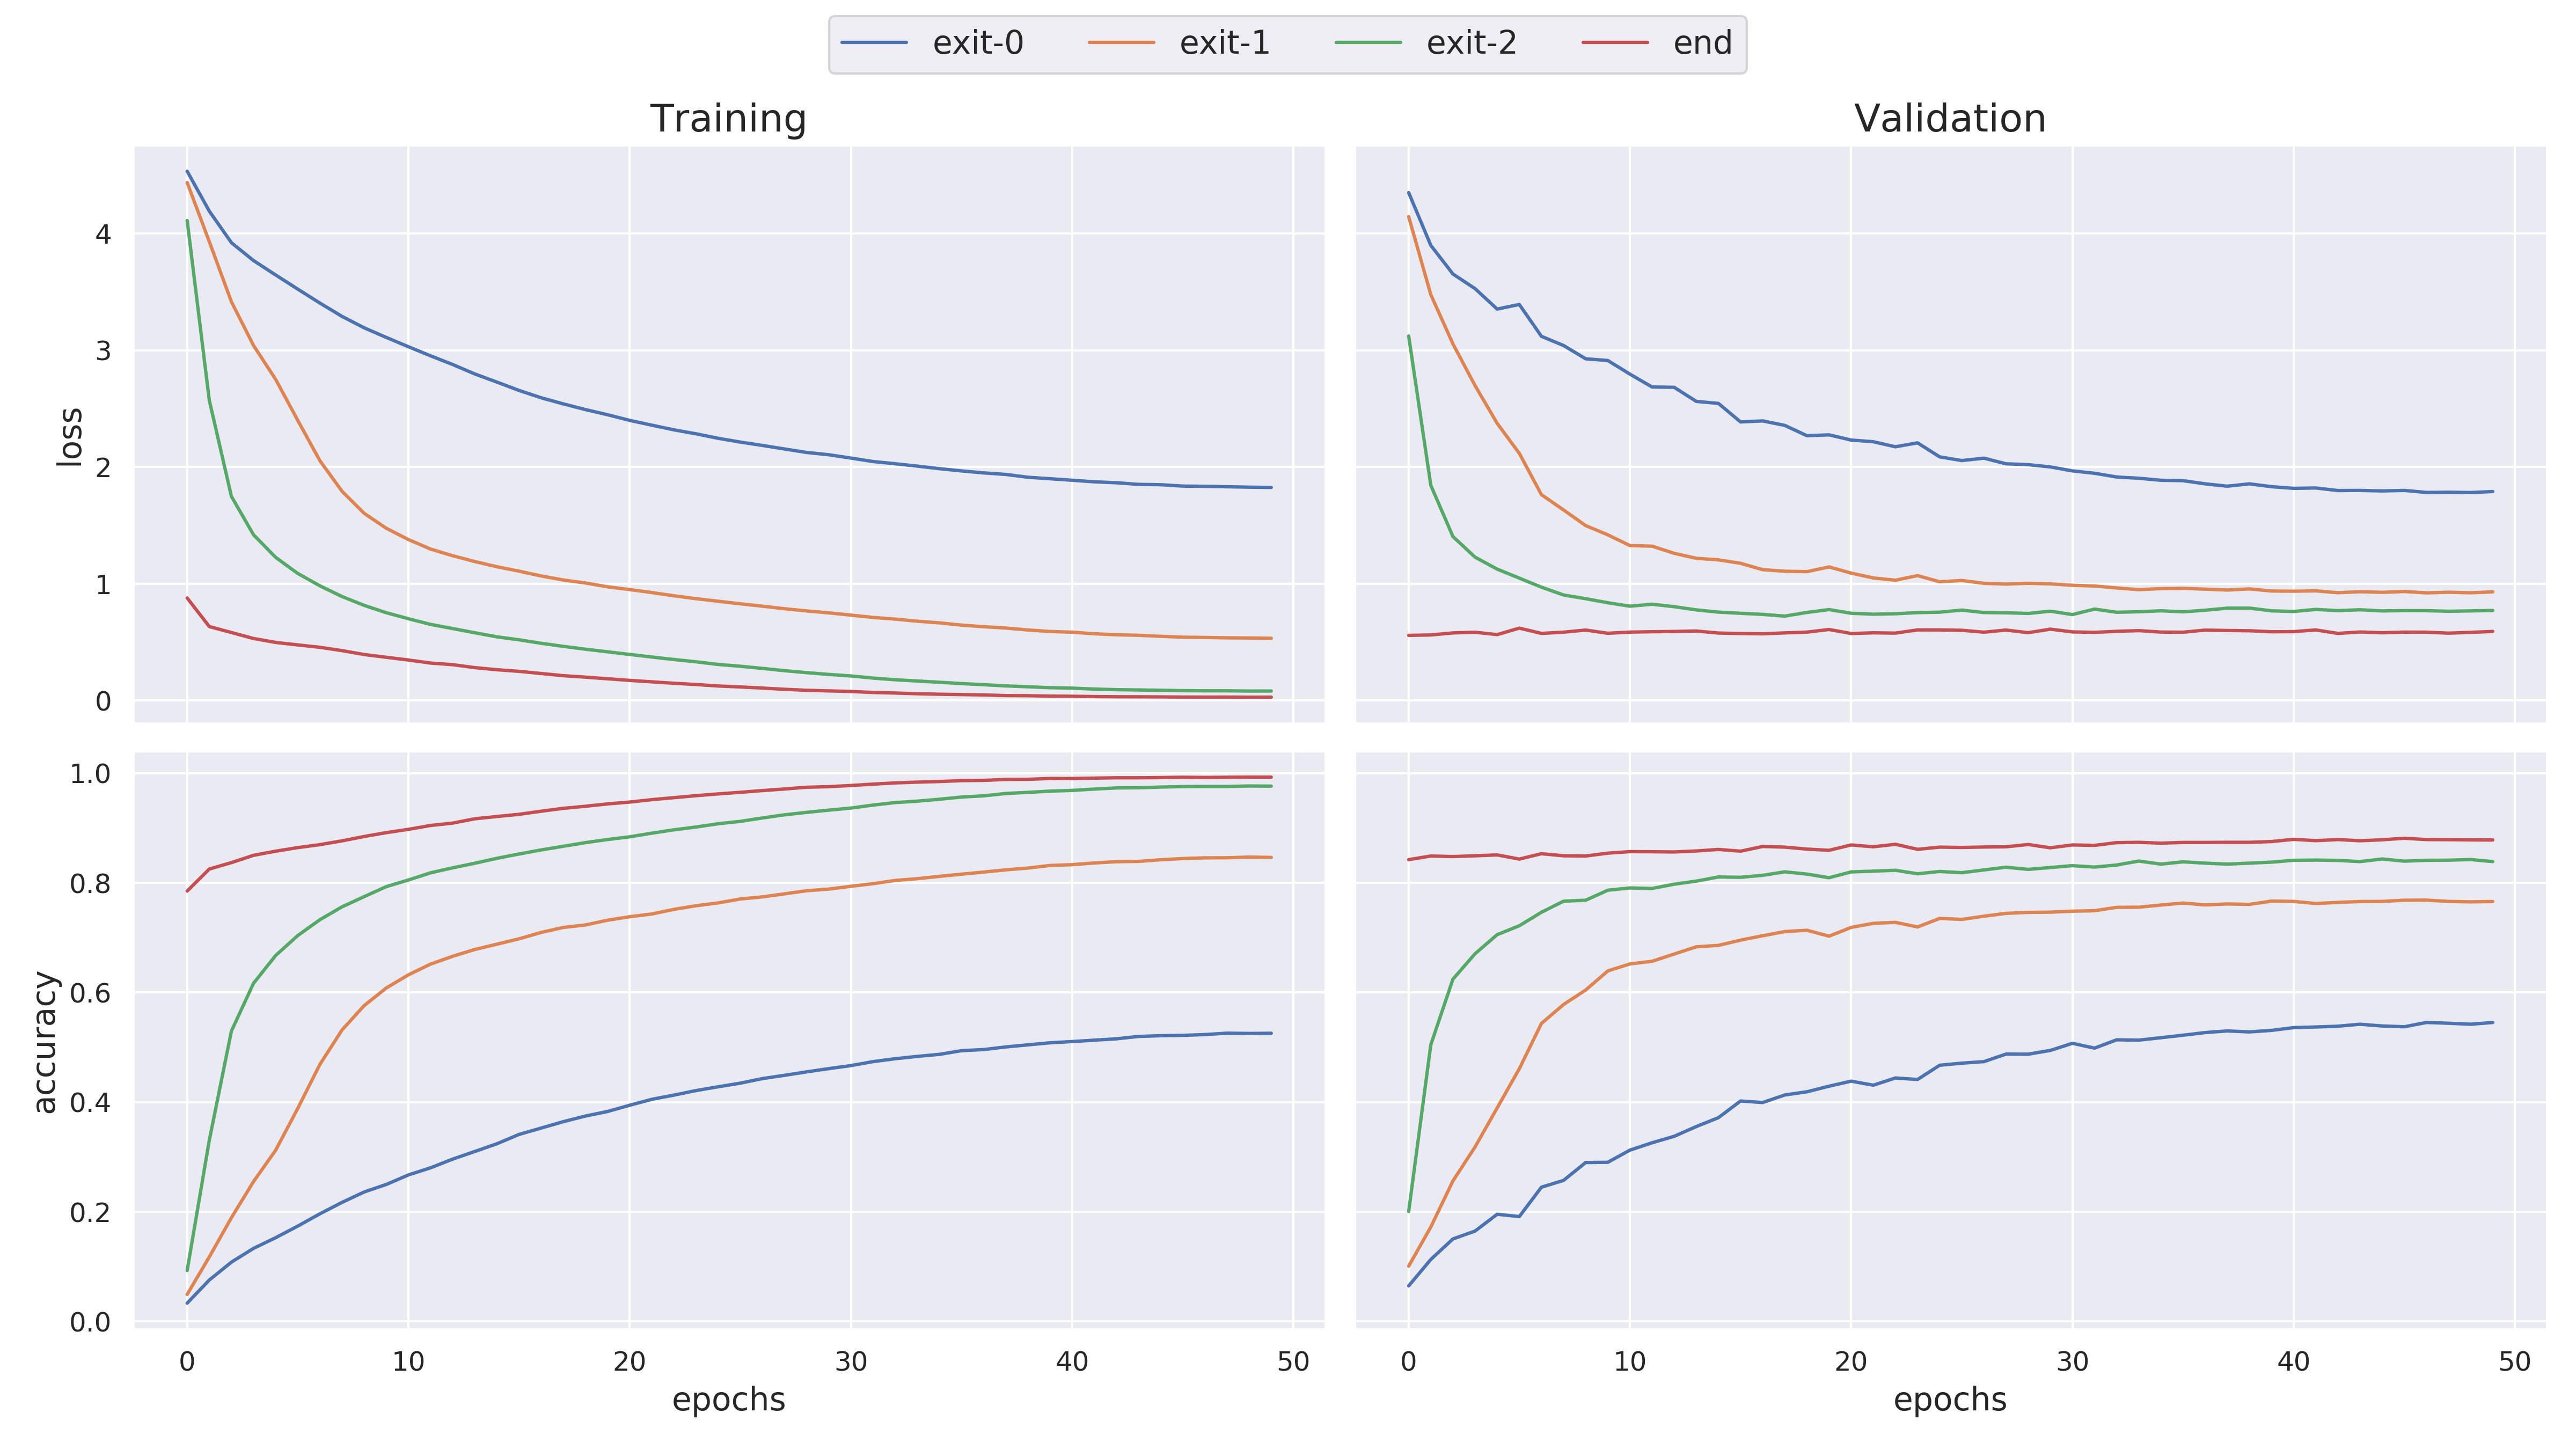
\includegraphics[width=\linewidth]{figures/training_plots/densenet_miniimagenet100}}
	\caption[Training progress of BrancyNets]{Training progress for \protect\subref{fig:B-resnet-miniimagenet100} B-ResNet and \protect\subref{fig:B-densenet-miniimagenet100} B-DenseNet} 
	\label{fig:b-net-miniimagenet-100}
\end{figure}


%\paragraph{Pascal VOC}
%
%\begin{figure}
%	\centering
%	\captionsetup[subfigure]{justification=centering}
%	\subfloat[Train loss\label{fig:B-resnet-voc-train-loss}]{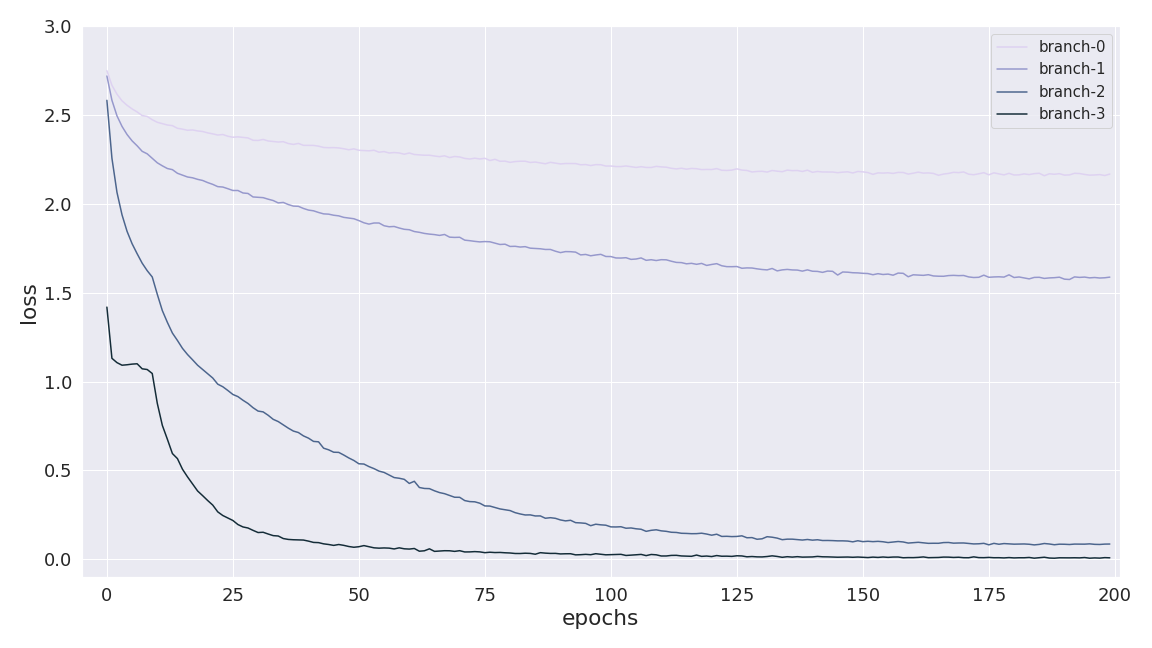
\includegraphics[width=.49\textwidth]{figures/BResNetVOC/BResNet_train_loss_VOC.png}}
%	\subfloat[Test loss \label{fig:B-resnet-voc-test-loss}]{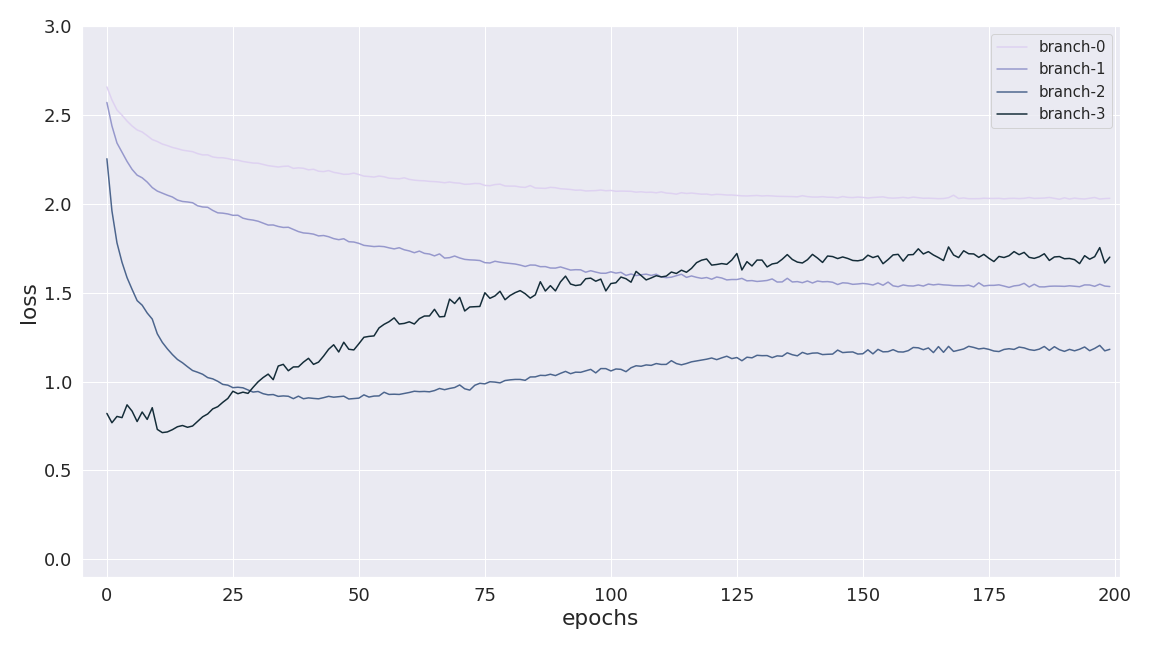
\includegraphics[width=.49\textwidth]{figures/BResNetVOC/BResNet_test_loss_VOC.png}}
%	\hfill
%	\subfloat[Train accuracy\label{fig:B-resnet-voc-train-acc}]{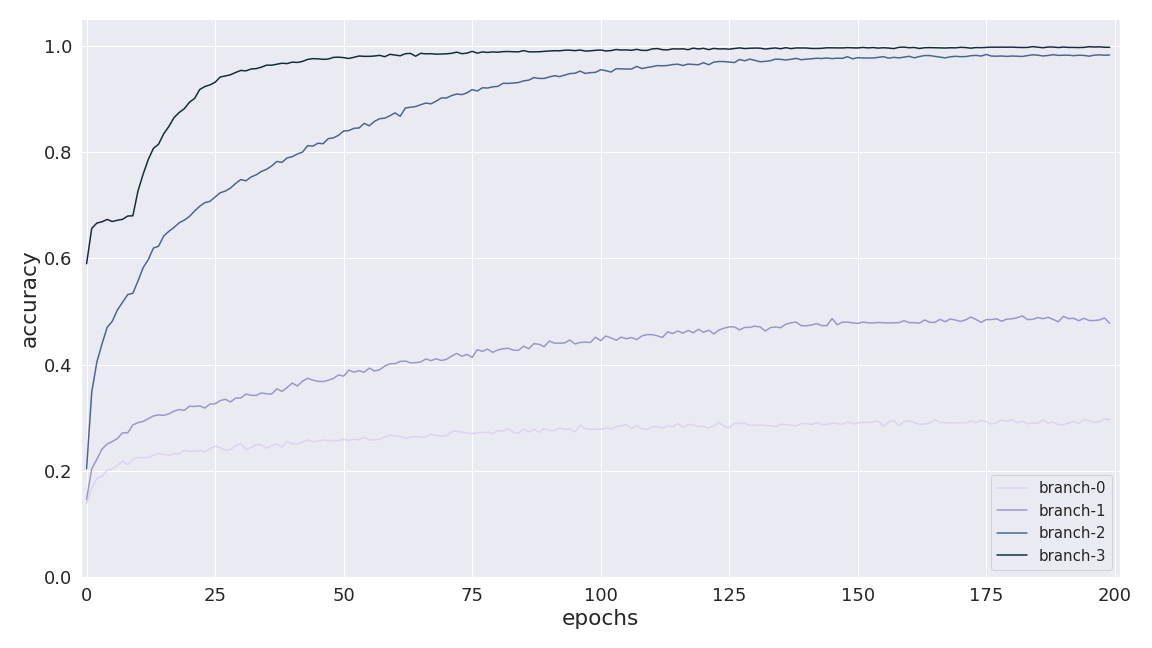
\includegraphics[width=.49\textwidth]{figures/BResNetVOC/BResNet_train_acc_VOC.png}}
%	\subfloat[Test accuracy\label{fig:B-resnet-voc-test-acc}]{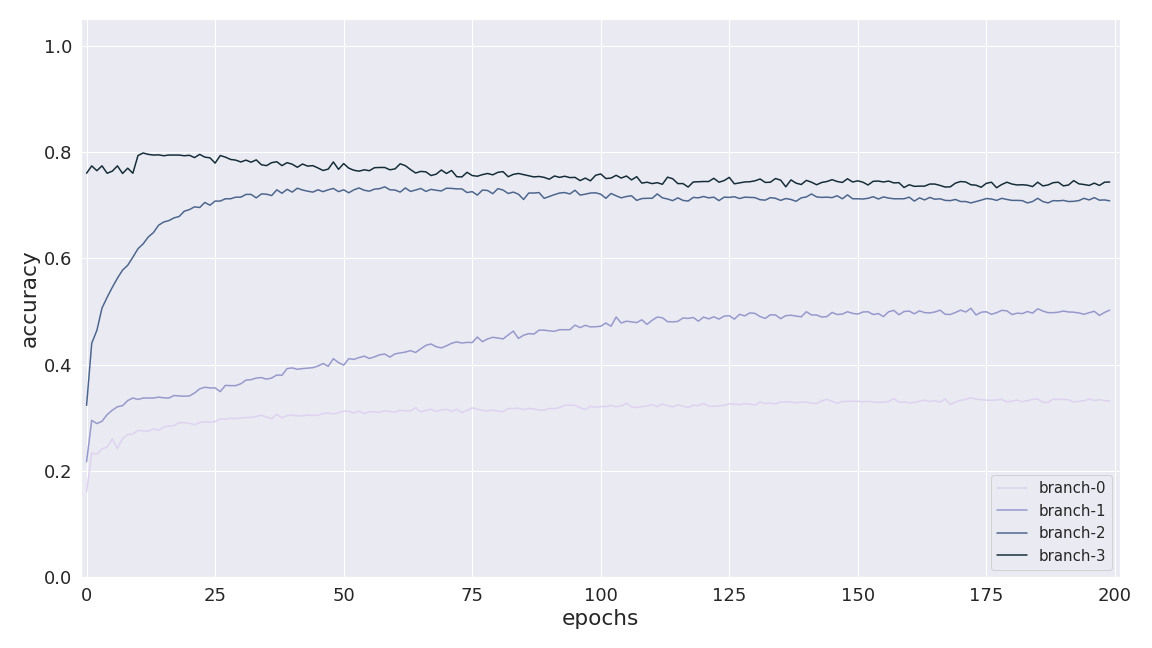
\includegraphics[width=.49\textwidth]{figures/BResNetVOC/BResNet_test_acc_VOC.png}}
%	\caption[B-ResNet VOC Training summary]{Training summary shows the progression of model attributes over times of epochs, \protect\subref{fig:B-resnet-voc-train-loss} train loss, \protect\subref{fig:B-resnet-voc-test-loss} test loss, \protect\subref{fig:B-resnet-voc-train-acc} train accuracy, \protect\subref{fig:B-resnet-voc-test-acc}, test accuracy.}
%\end{figure}
%
%Visualizing the training progression, clearly indicates that model overfitting to the training data. When a model overfits it suffers to generalize the true underlying distribution of the data. This can be caused by insufficient number of training samples or too complex a model. Since the model has shown promising results in image classification task previously, we can conclude, that the dataset is too sparse.
%
%Even though the model fails to generalize, the experiment still produce interesting results. Given an early exiting model as B-ResNet 50\% of the test samples can be correctly classified using only half of the \gls{dnn}.

\section{Inference Time Analysis}

\begin{figure}
	\captionsetup[subfigure]{justification=centering}
	\centering
	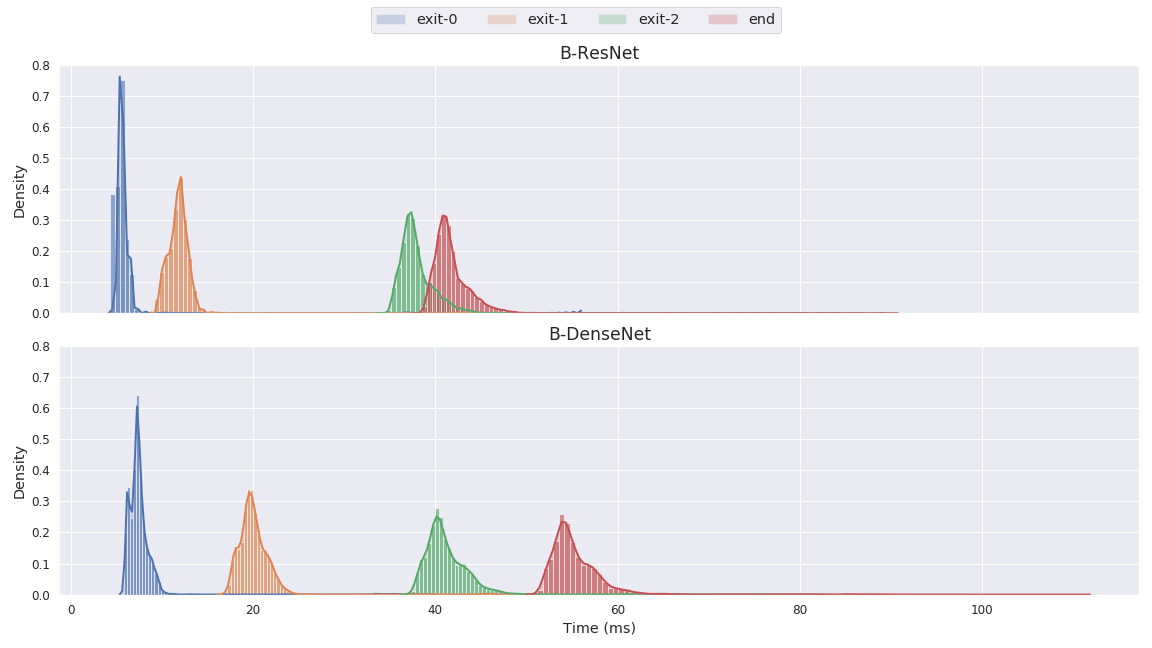
\includegraphics[width=\linewidth]{figures/threshold_plots/timing}
	\caption[Inference Analysis]{Inference Analysis}
\end{figure}

\section{Threshold Analysis}

In this experiment the MiniImageNet100 validation set have been used to evaluate the two threshold metrics; \emph{Confidence Threshold} and \emph{Score-Margin Threshold}. Figure \ref{fig:thresholds} compares the performance of each exit on all samples.

\begin{figure}
	\captionsetup[subfigure]{justification=centering}
	\centering
	\subfloat[ResNet\label{fig:threshold_resnet}]{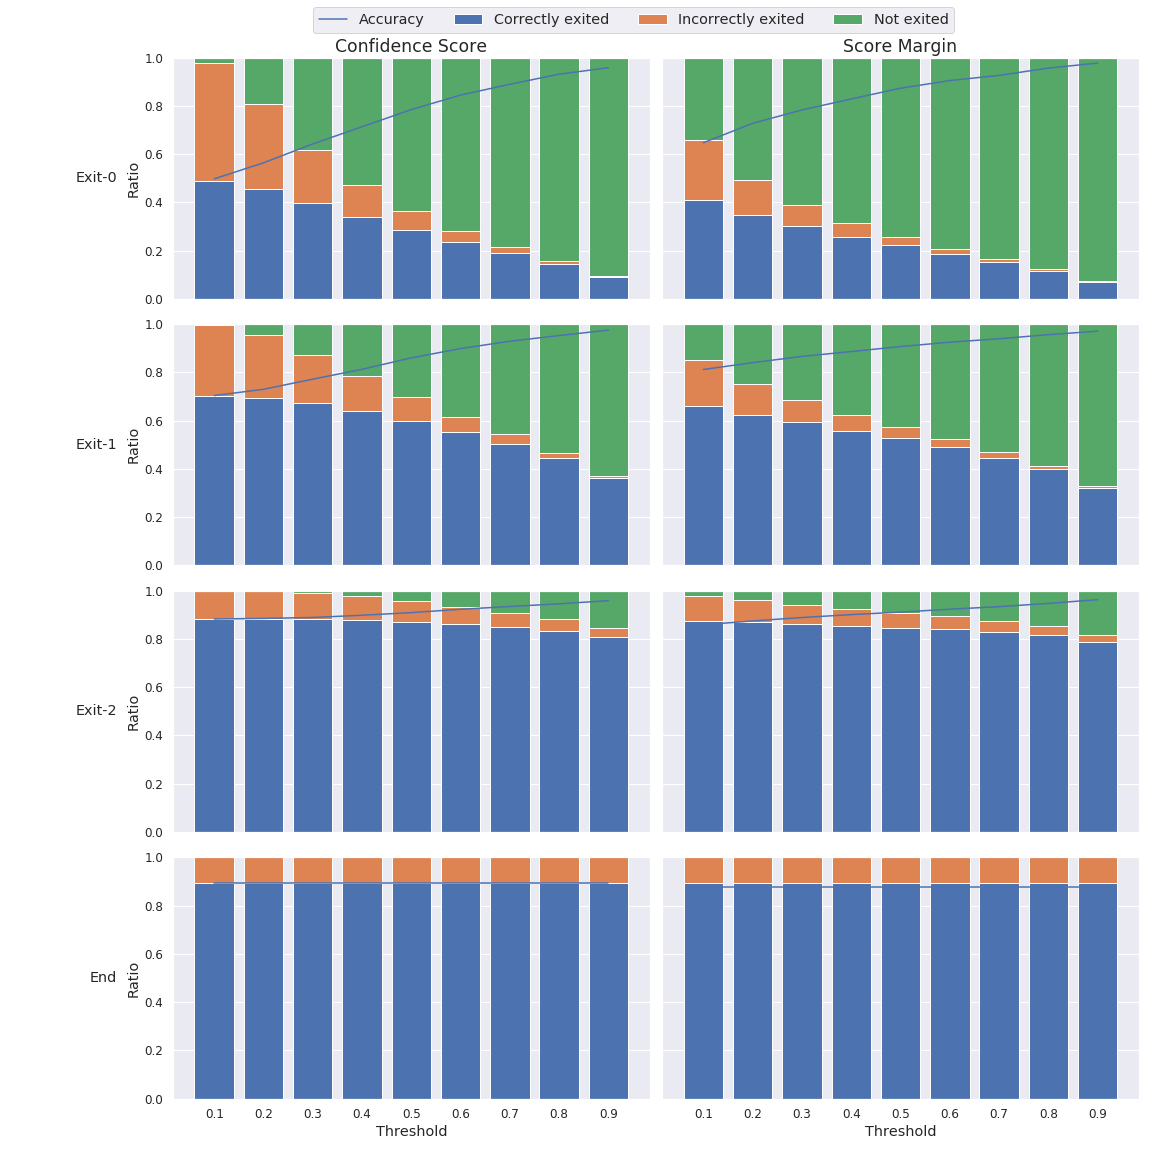
\includegraphics[width=\linewidth]{figures/threshold_plots/threshold_analysis_resnet101}}

\end{figure}
\begin{figure}
	\captionsetup[subfigure]{justification=centering}
	\centering
%	\subfloat[ResNet\label{fig:threshold_resnet}]{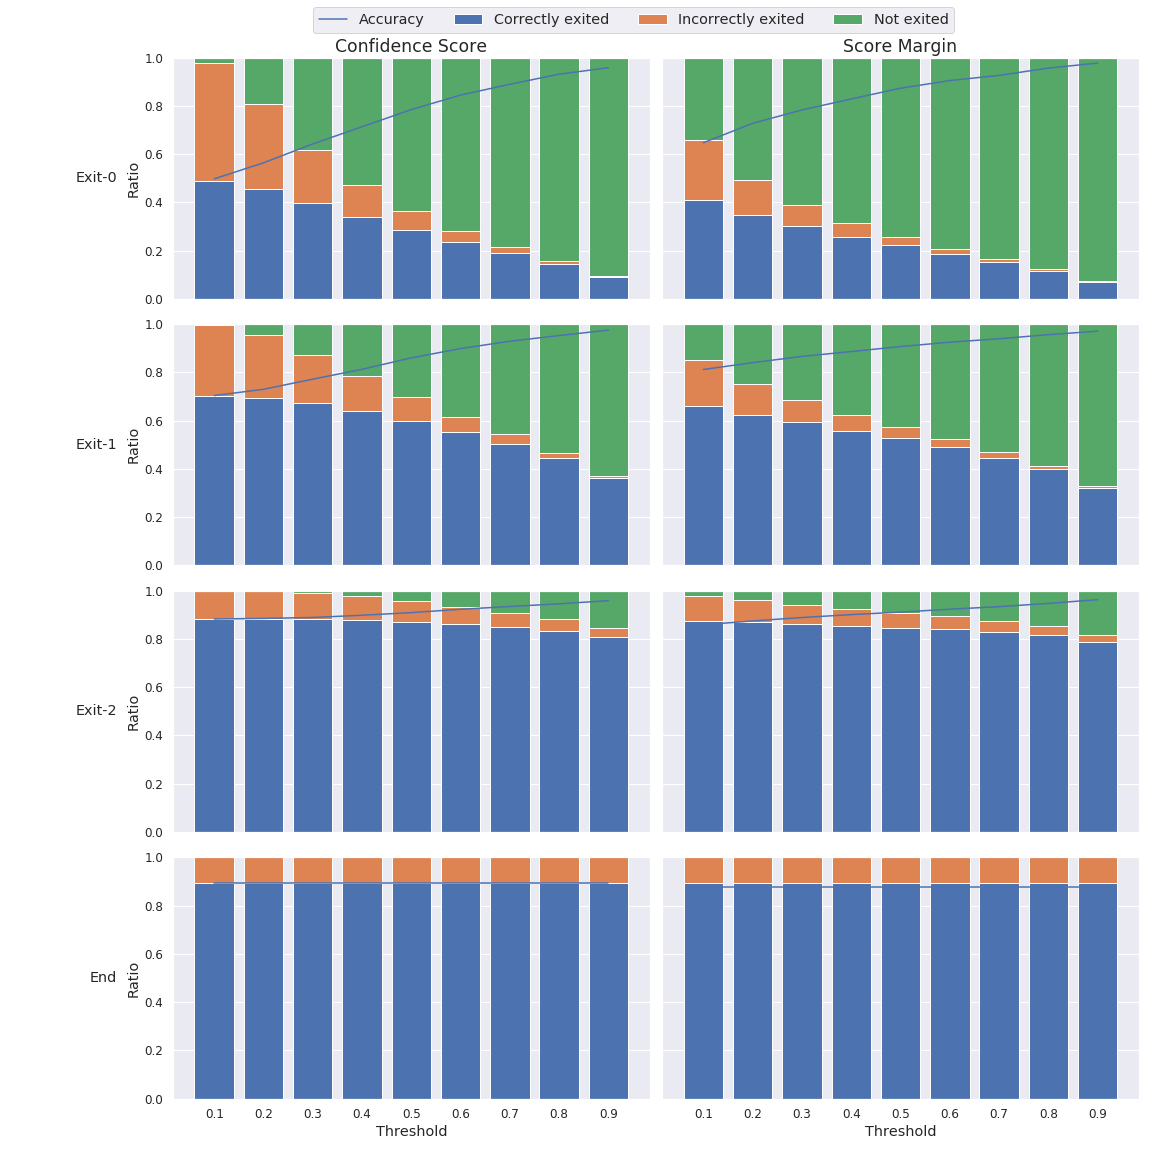
\includegraphics[width=.8\linewidth]{figures/threshold_plots/threshold_analysis_resnet101}}
	\subfloat[DenseNet\label{fig:threshold_densenet}]{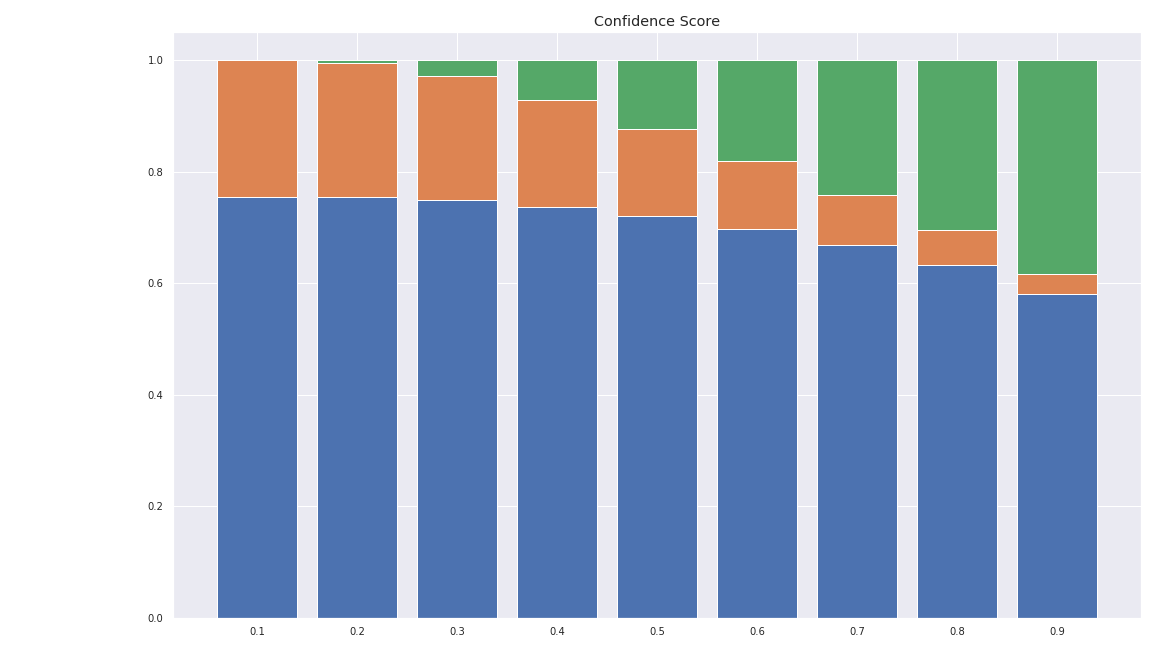
\includegraphics[width=\linewidth]{figures/threshold_plots/threshold_analysis_densenet100}}
	\caption[Threshold Comparison]{Threshold comparison of confidence threshold and score margin threshold.}
	\label{fig:thresholds}
\end{figure}

The \emph{score-margin} has more desirable traits, as less samples are incorrectly exited at lower threshold, only at the expense of a few additional samples not exited. Thus more suitable for application, that can slack a bit on accuracy to meet a latency constraint. Henceforth the \emph{score-margin} threshold are used.

\begin{figure}
	\centering
	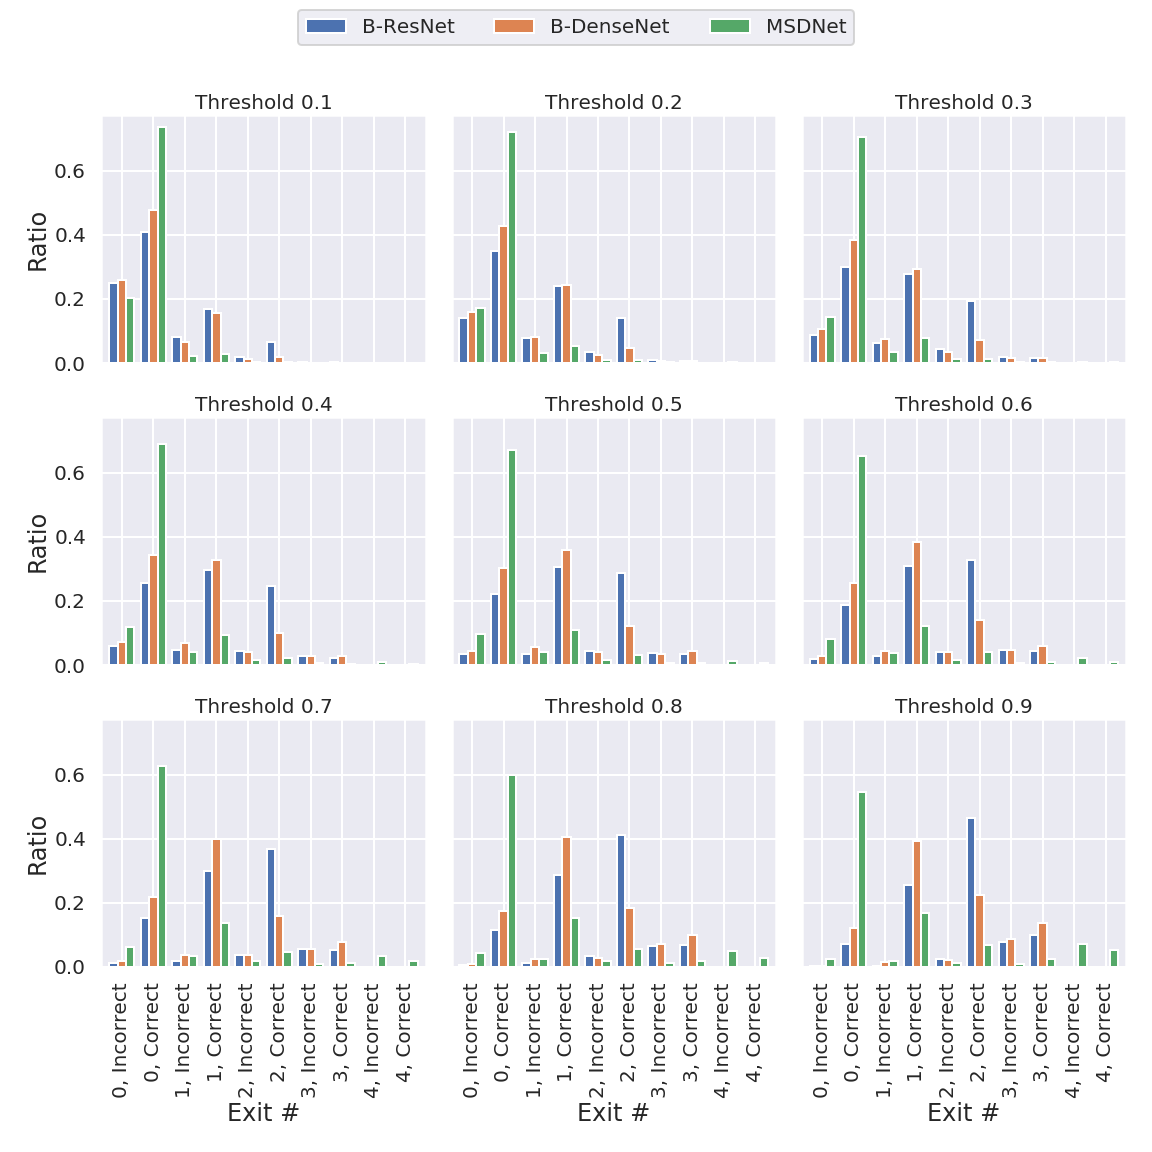
\includegraphics[width=\linewidth]{figures/threshold_plots/inference_threshold_test}
	\caption{Score-Margin Exiting}
	\label{fig:inferencethresholdtest}
\end{figure}

\section{Early Exiting vs. Conventional Inference}

Conventional versions of the \gls{dnn}'s were trained on the \gls{min100}. The model were initialized with ImageNet weights. The models' feature extractor was frozen, hence only the classifier was trained. The models were used to compare with early exiting inference accuracy and latency, see figure \ref{fig:early_exit_vs_conv}.

  \begin{figure}
  	\captionsetup[subfigure]{justification=centering}
  	\centering
  	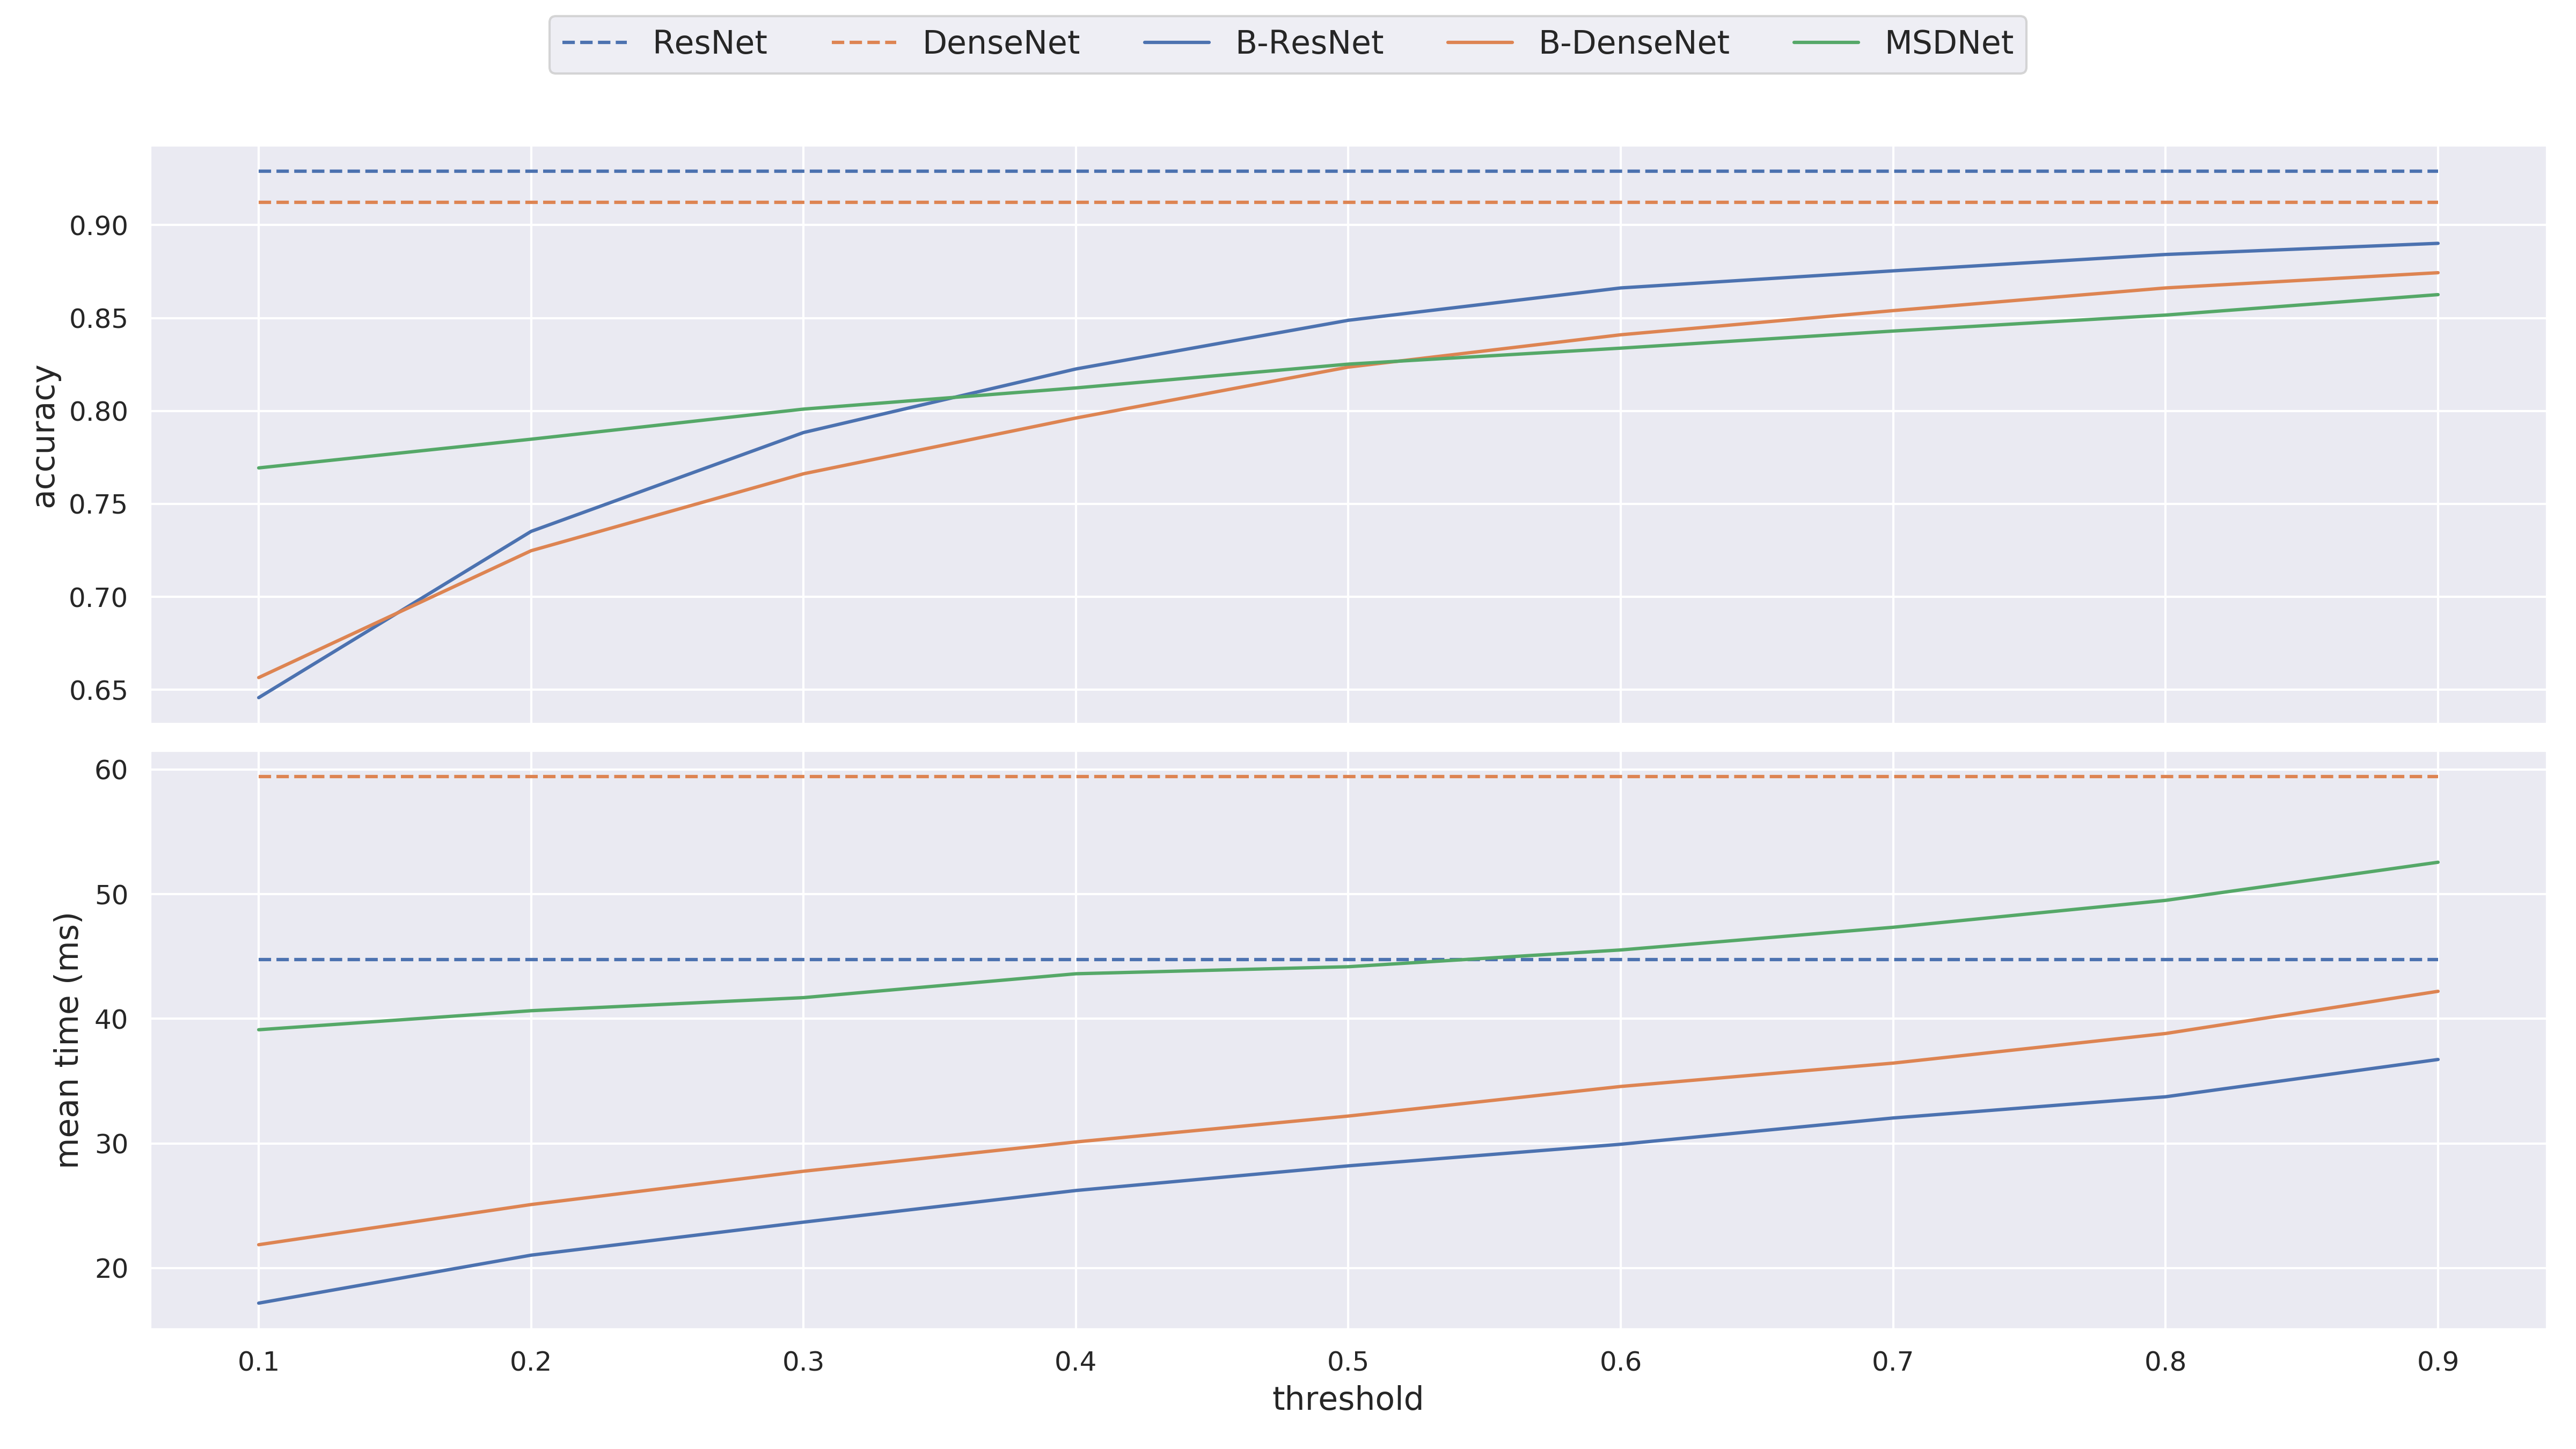
\includegraphics[width=\linewidth]{figures/threshold_plots/compare_exiting_vs_no_exiting}
  	\caption[Architectural Comparison]{Architectural Comparison}
  	\label{fig:early_exit_vs_conv}
  \end{figure}

The figure clearly states the accuracy-latency trade-off imposed by early exiting. The conventional models are clearly more accurate, however also expectantly slower, than their more flexible exiting counterpart. B-\gls{densenet} benefits more from early exiting, when a threshold of 0.9 is chosen, it gives up 4 percentage point in accuracy and reducing inference latency by 29 \%. The B-\gls{resnet} have about the same compromise in terms of accuracy, however only a reduction of 18 \% inference latency. B-\gls{resnet} still perform better in terms of both accuracy and inference time. The \gls{resnet}. 

\section{Transport Protocol} 

Offloading tasks over the network, irregardless fully or partially requires a transport protocol. The selection is typically a choice of either \gls{tcp} or \gls{udp}. \gls{tcp} is a reliable protocol, that guarantee no losses by retransmission of lost packets. \gls{udp} on the other hand is a best-effort protocol, that accept packets loss, thus not introducing retransmission communication overhead. 


Fully offloading \gls{jpeg} compressed images for classification require no losses for human-readability. Sending intermediate features of a \gls{dnn} may not be as intolerant to losses and might be able to function with the far more lightweight \gls{udp}. In current research literature the choice of \gls{tcp} seems given in advance.  

In this experiment the \gls{tcp} transmission time and retransmission rate is investigated under different communication environments. 

\begin{figure}
	\centering
	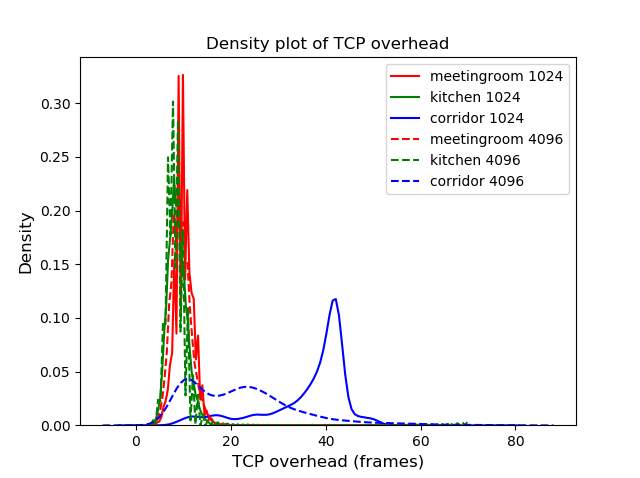
\includegraphics[width=\linewidth]{figures/tcp/tcpoverhead}
	\caption[TCP retransmission overhead]{TCP retransmission overhead}
\end{figure}